\chapter{Equational Reasoning on x86 Assembly} \label{chapter:equational_reasoning}
\section{Algebra of Program} \label{sec:algebra_of_program}
\paragraph{}
One might reason about an equation to decide whether it is a consequence of an equational system (i.e. a set of equations), but that is not the only application of equational reasoning. In the context of computer science, and more precisely, in the context of pure functional programming languages, one could see his or her code as an equation made of smaller equations that have been glued together with special operators. It would then be possible to apply rewriting rules to change the representation of the code~\cite{htfet1980equations}. One example would be to replace a function call by its body, or the body by a function call. A simple example of this can be observed in Listing~\ref{lst:haskell_eq_rewriting}. One could go further by adding a function making a call on any of the three functions, with concrete parameters, and reduce it to a single integer value. \\

\begin{lstlisting}[caption={Example of equational reasoning in Haskell.}, label={lst:haskell_eq_rewriting}, frame=tlrb, language={Haskell}]
square :: Integer -> Integer
square x = x * x

pythagoras :: Integer -> Integer -> Integer
pythagoras a b = square a + square b

-- Replacing the square definition by its body
pythagoras' :: Integer -> Integer -> Integer
pythagoras' a b = a * a + b * b
\end{lstlisting}

\paragraph{}
This algebra of programs (also called equational reasoning) is a technique that has emerged from the functional programming world in response to the problem of proving program correctness. Its strength resides in the fact that, contrary to most formal program solving methods, an average programmer is able to prove the correctness of his or her (functional) programs without requiring to master a panoply of advanced mathematical and logical concepts~\cite{backus1978can}. Indeed, a programmer would use his or her programming knowledge of the language to derive proofs, just like one would do with algebraic proofs.

\paragraph{}
For this algebra of programs to work, it requires the underlying language to be purely functional, that is, to not allow variables to mutate. Indeed, if they were allowed to change their states, the order of evaluation (reduction) would have an impact on the semantic of the code. An implication of this property is the gain of what is called referential transparency. It can be informally explained as $f(x) = f(x)$: A function, when applied to the same parameters over time, will always give back the same result. A consequence of this property is that every function applications to the same parameters can be replaced by their result. This property will not hold on for imperative languages. Indeed, being able to write functions that rely on mutable global variables to produce their output clearly contradicts the stated property.

\paragraph{}
Proving correctness is not the only benefit of equational reasoning. Richard Bird, the author of the book titled \textit{Pearls of Functional Algorithm Design}~\cite{bird2010pearls}, shows how equational reasoning can be used to design efficient algorithms. Starting from an obviously correct but inefficient version of an algorithm, he iteratively rewrites it until reaching a optimised version.

\section{Equational Reasoning of x86 Assembly Code} \label{sec:eqr_of_x86_assembly_code}
\paragraph{}
This section is entirely based on the paper titled \textit{Equational Reasoning of x86 Assembly Code}~\cite{coogan2011equational} written by Kevin Coogan and Saumya Debray from the University of Arizona. The reason this work takes such a central place is that my contribution presented in Chapter~\ref{chapter:contribution} is based on their work.

\paragraph{}
The paper argues that there is a myriad of source code analysis tools focused on analysing correctness, efficiency and security of software application at source code level, but that there is a void for similar tools aimed at assembly code (either from disassembly or hand written sources). To overcome this problem, they developed a prototype which is able to perform dynamic analysis on assembly code for the Intel x86 architecture by means of equational reasoning. It works by first translating every instruction into a set of equations which encapsulates their exact semantic to form an equational reasoning system, and then manipulating the system in various ways to extract meaningful information.

\paragraph{}
Equational reasoning over assembly code is a novel application of equational reasoning. It has been chosen by the authors for it allows to accurately model the dependencies between instructions, which could be lost with other analysis tools. The dependencies arise from the many registers' names and the implicit side effects most instructions have. Moreover, equational reasoning allows to improve the readability of the assembly code. These three topics are discussed in a more detailed manner below.

\begin{itemize}
	\item \textbf{Register Name Aliasing}: As explained in Section~\ref{sec:registers}, the four all purpose registers can be addressed in four different ways: As a whole, as the bottom 16 bits, and as the left half and the right half of the bottom 16 bits. This has been illustrated in Figure~\ref{fig:register_name_aliasing}. The equational representation allows to modelise the relationship between a register and its many names to provide a more accurate analysis.    
	\item \textbf{Side Effects}: Most instructions have side effects on the $eflags$ register. For example, the add instruction will set the overflow flag to one if the arithmetic operation has overflowed. This register is then used to influence the instructions in charge of the conditional branching. When translating an instruction into a set of equations, a subset of the set will be dedicated to representing this behaviour. 
	\item \textbf{Readability}: Because assembly languages are the lowest level of abstraction one could reach, they can be very verbose. A simple operation in a high level language will be translated into a set of many assembly instructions, making it harder to read, and so, to reason out. As a result, being able to visualise these instructions in a straight forward manner is of substantial help to reverse engineers. This can be arguably achieved by the use of an equational representation.
\end{itemize}

\begin{figure}[!htb]
	\centering
	\includegraphics[width=0.3\textwidth]{equational_reasoning/register_name_aliasing.png}
	\caption{$r = {A, B, C, D}$. Illustrates the dependencies between a register and its sub-parts.}
	\label{fig:register_name_aliasing}
\end{figure}

\paragraph{}
As for the choice of using the Intel x86 architecture, it comes from the fact that the authors intended to use their tool to analyse malware, which is usually written to target the most ubiquitous architecture. To be noted that one could easily extend their research by adding support for the x64 architecture, something that will not be discussed in this work.

\subsection{Motivating Example}
\paragraph{}
To illustrate what has been discussed so far, an example given by Kevin Coogan in his PHD thesis titled \textit{Deobfuscation of Packed and Virtualization-Obfuscation Protected Binaries}~\cite{coogan2011deobfuscation} will be presented and broadly explained. The reason for this example to not be an original one is due to the fact that, at least to my knowledge, the tool made by the authors has not been released to the public. To be noted that the vocation of this example is not to exhaustively explain everything in detail, but rather to give a broad idea of why equational reasoning is helpful for performing reverse engineering.

\paragraph{}
The x86 assembly trace given in Listing~\ref{lst:equational_reasoning_example_asm} will be the input given to the tool. It performs operations on three registers, $eax$, $ebx$, and $ecx$. For this example, we are only interested in the value that $eax$ will take once past the fifth instruction. 

\paragraph{}
The Figure~\ref{fig:equational_reasoning_example_after} shows the equations that have been generated from the trace. All left-hand side terms in the equation listing have a subscript which relates to the line numbers in the trace, and the right-hand side terms have subscripts relating to previous results of equations. The $const$ subscript notifies that no previous information is known about an operand. One can see how the one-to-many mapping between instructions and equations allows to fully modelise the behaviour of each instruction. One might also have noticed that the very last instruction has been added manually. Because we are interested in the content of $eax$ and not just $ax$, adding this equation allows the analysis to be performed in the whole register.

\paragraph{}
Finally, Figure~\ref{fig:equational_reasoning_example_final} shows how the equational reasoning is applied. We start by saying that $eax_6 = eax_5$ and recursively substitute the terms by their definition found in Figure~\ref{fig:equational_reasoning_example_after}. Simplifications are performed whenever possible until reaching an irreducible expression, here $eax_6 = 0x1$. \\

\begin{lstlisting}[caption={Snippet of assembly code. From the PHD thesis of Kevin Coogan~\cite{coogan2011deobfuscation}.}, label={lst:equational_reasoning_example_asm}, frame=tlrb, language={[x86masm]Assembler}]
0: xor ebx, ebx
1: not bx
2: mov eax, 0x7e5bd96f
3: mov ecx, 0x81a42692
4: and eax, ecx
5: add ax, bx
\end{lstlisting}

\begin{figure}[!htb]
	\centering
	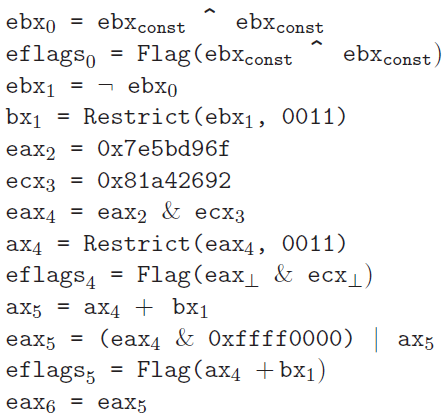
\includegraphics[width=0.5\textwidth]{equational_reasoning/equational_reasoning_example_after.png}
	\caption{Equational system generated from the trace found in Listing~\ref{lst:equational_reasoning_example_asm}.}
	\label{fig:equational_reasoning_example_after}
\end{figure}

\begin{figure}[!htb]
	\centering
	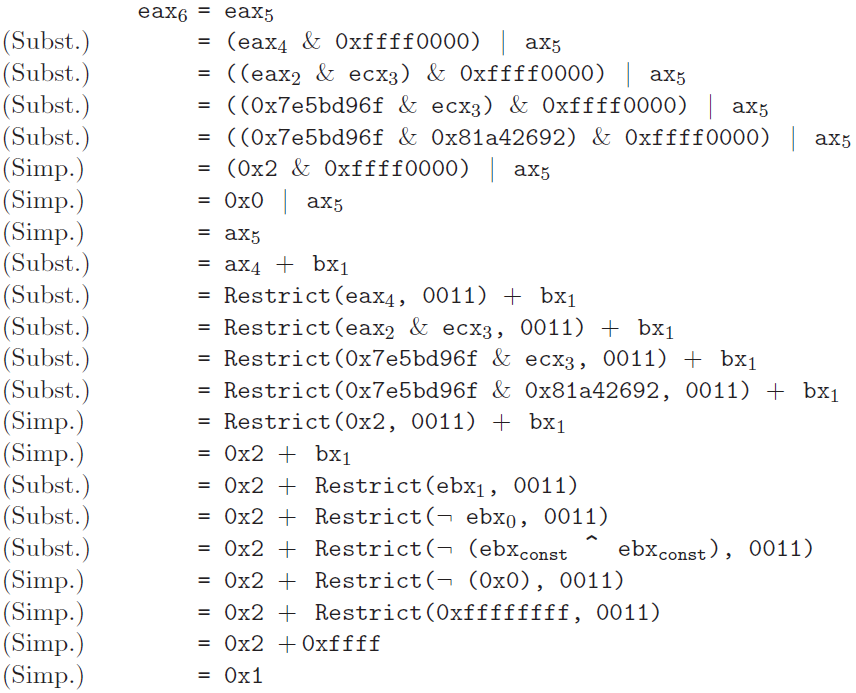
\includegraphics[width=0.85\textwidth]{equational_reasoning/equational_reasoning_example_final.png}
	\caption{Simplification of an equation about the $eax$ register. From the PHD thesis of Kevin Coogan~\cite{coogan2011deobfuscation}.}
	\label{fig:equational_reasoning_example_final}
\end{figure}

\pagebreak

\subsection{Notation}
\paragraph{}
As said in Section~\ref{sec:instructions}, the syntax of the Intel x86 ISA is as follows:\\
\textit{label: mnemonic argument1, argument2, argument3}\\
Most of the instructions have an arity less than or equal to 2 and use the first operand as a source and destination operand. For example, the multiplication instruction $mul\ arg1,\ arg2$ could be rewritten as $arg1 := arg1 * arg2$. An operand can be a register name, a constant (also called immediate value), or a memory location represented with an address expression. The expression is found enclosed in brackets and has to be evaluated before being used. For example, the instruction $mov\ eax,\ [ebx+8]$ will take the value at the address stored in $ebx$ plus $8$ and store it into $eax$.

\paragraph{}
Now it will be discussed the notation for the equations. Each instruction's mnemonic will be mapped onto an operator that can be more easily understood whenever it is possible. Source operands can then be applied to the operator using either infix or prefix notation and it will give back a result called the destination operand. This is what has been done with the $mul$ example from the previous paragraph. Just like with assembly instructions, an operand can either be a constant, a register name, or a memory expression. For the latest case, a memory expression will be represented by $MLOC[a..b]$, where $a..b$ defines a memory range, and the value stored at the memory location will be represented by $ValueAt(MLOC[a..b])$.

\paragraph{}
Registers and memory locations will change their state over time, something that is not compatible with the ideas proposed by the authors so far. To get over this issue, every variable (either registers or memory location) is given an identifier to uniquely identify every state it has had. This will be done via the use of subscripts. The line number of each instruction in the trace will be referred as the order number and will be used as a source for unique identifiers.

\paragraph{}
A simple example showing the new notation can be observed below. In Listing~\ref{lst:notation_example_1} it is shown a trace prefixed with line numbers, in Listing~\ref{lst:notation_example_2} the generated equations. The $mov$ is replaced by an equal sign, and the $add$ by a plus sign. To be noted that, for the purpose of this example, the equations do not fully modelise the instructions. \\

\begin{lstlisting}[caption={A sample of trace.}, label={lst:notation_example_1}, frame=tlrb, language={[x86masm]Assembler}]
0: mov eax, [401000]
1: add eax, 2
\end{lstlisting}

\begin{lstlisting}[caption={A partial translation of the trace from Listing~\ref{lst:notation_example_1}.}, label={lst:notation_example_2}, frame=tlrb, language={[x86masm]Assembler}]
<@$eax_0 := ValueAt(MLOC[40100..401003])_{const}$@>
<@$eax_1 := eax_0 + 2$@>
\end{lstlisting}


\subsection{Implementation}
\subsubsection{Translating Instructions} \label{sec:translating_instructions}
\paragraph{}
Each instruction has to be converted into a set of equations which fully modelise the behaviour of the instruction. To do so, the tool will linearly pass over the trace and perform the translation. The order number of each instruction will be used as a unique identifier for the destination operands (left-hand side) of its generated set of equations. As for the source operands, since nothing is known about them yet, the bottom ($\bot$) symbol will be used instead. This will be replaced by valid identifiers later on when dependencies are being resolved.

\paragraph{}
The $push$ and $div$ instructions will be used as examples to illustrate the conversion. In the situation where $push\ eax$ is seen as a complete trace, the following set of equations will be generated: \\
\begin{lstlisting}[frame=tlrb, language={[x86masm]Assembler}]
<@$ValueAt(MLOC[1000..1003])_0 := eax_{\bot}$@>
<@$esp_0 := esp_{\bot} - 4$@>
\end{lstlisting}


\paragraph{}
The stack is simply a special usage of the memory combined with dedicated registers. Putting the value manually on top of the stack (at address $1000$ in this example) and updating the stack pointer register to the newest top position is equivalent to using $push$. If $div\ eax, 2$ were seen as a complete trace, the following equations would be generated: \\
\begin{lstlisting}[frame=tlrb, language={[x86masm]Assembler}]
<@$eax_0 := eax_{\bot} / 2$@>
<@$eflags_0 := Flag(eax_{\bot} / 2)$@>
\end{lstlisting}

\paragraph{}
Here, the $eflags$ register has to be updated because 6 flags can possibly be changed. This is done thanks to the new equation $Flag$, which takes the expression as the only source operand.

\subsubsection{Resolving Dependencies}
\paragraph{}
Here it will be discussed how the bottom symbols are replaced by identifiers to resolve the dependencies between the equations. This process is not straight forward for two reasons, the first one being that registers can be accessed using different names to read and write different parts of them, and the second one from the fact that the Intel x86 architecture is byte addressable.

\paragraph{}
Resolving dependencies will be done by going backward through the listing of equations and looking where the source operands have been declared. There are five scenarios that the algorithm must handle to correctly resolve the dependencies. They will be described in the list below, and an example for each scenario can be found in Table~\ref{table:resolving_dependencies}.

\begin{enumerate}
	\item \textbf{First case}: A source operand is fully defined by a previous destination operand. In this case, the source operand will simply take the identifier of the destination operand.
	\item \textbf{Second case}: A source operand is a subset of another destination operand. For registers, it could be $ch$, which is a subset of $ecx$, and for memory location, it could be $MLOC[1000..1001]$, which is a subset of $MLOC[1000.10003]$. Because they are not equal, it is required to refine the most general operand to match the other one. This is done with the $Restrict$ equation, which takes 2 operands, a register or memory location, and a mask to tell which part to isolate. When scanning backward for the definition of an operand, the tool will then have to detect when this case applies and add the $Restrict$ equation with a correct mask.
	\item \textbf{Third case}: It is the opposite of the second case. A source operand is defined by multiple previous destination operands. For example, $ah$ and $al$, which defines $ax$. To handle this situation, the tool has to detect the parts that form the whole and add equations to each of them to progressively recompose the whole. This can be observed in line 3 and 4 from the example.
	\item \textbf{Fourth case}: A source operand is made from parts of multiple destination operands while none is a subset of the other. This is impossible for registers but not for memory locations. To deal with this case, it is necessary to combine the solutions of the second and third case.
	\item \textbf{Fifth case}: When a source operand cannot be traced to a destination operand, nothing can be said about it. In this case, the identifier will be $const$. This can happen at the beginning of the program when the registers have not been initialised yet and also when dealing with obfuscated code.
\end{enumerate}

\begin{table}[!htb]
	\centering
	\begin{tabular}{|l|l|l|}
		\hline
		Case & Before & After \\ \hline \hline
		1:  & $\begin{array} {lcl} eax_0 := 40 \\ eax_1 := eax_{\bot} + 2 \end{array}$ &  $\begin{array} {lcl} eax_0 := 40 \\ eax_1 := eax_{0} + 2 \end{array}$ \\ \hline
		2:  & $\begin{array} {lcl} eax_0 := FFFFh \\ ah_1 := ah_{\bot} \oplus bh_{\bot} \end{array}$       & $\begin{array} {lcl} eax_0 := FFFFh \\ ah_0 := Restrict(eax_0, 0010) \\ ah_1 := ah_{ah_0} \oplus bh_{cons} \end{array}$ \\ \hline
		3:  & $\begin{array} {lcl} eax_0 := 4000 \\ ah_1 := 10 \\ al_2 := 10 \\ eax_3 := eax_{\bot} + 2 \end{array}$       & $\begin{array} {lcl} eax_0 := 4000 \\ ah_1 := 10 \\ eax_1 := (eax_0 \& 0010) | ah_1 << 6 \\ al_2 := 10 \\ eax_2 := (eax_1 \& 0001) | al_2 \\ eax_3 := eax_{2} + 2 \end{array}$      \\ \hline
		4:  & $\begin{array} {lcl} ValueAt(MLOC[0..3])_0 \\ \quad := FFFFh \\ ValueAt(MLOC[4..7])_1 := \\ \quad FFFFh \\ eax_2 := ValueAt(MLOC[2..5])_{\bot} \end{array}$       & $\begin{array} {lcl} ValueAt(MLOC[0..3])_0 := \\ \quad FFFFh \\ ValueAt(MLOC[2..3])_0 := \\ \quad Restrict(ValueAt(MLOC[0..3])_0, 0011) \\ ValueAt(MLOC[4..7])_1 := \\ \quad FFFFh \\  ValueAt(MLOC[4..5])_1 := \\ \quad Restrict(ValueAt(MLOC[4..7])_1, 1100) \\ ValueAt(MLOC[2..5])_1 := \\ \quad (ValueAt(MLOC[2..3])_0 << 16) \\ \quad | ValueAt(MLOC[4..5])_1 \\ eax_2 := ValueAt(MLOC[2..5])_{1} \end{array}$      \\ \hline
		5:  & $\begin{array} {lcl} eax_0 := ebx_{\bot} + ecx_{\bot} \end{array}$       & $\begin{array} {lcl} eax_0 := ebx_{const} + ecx_{const} \end{array}$      \\ \hline
	\end{tabular}
	\caption{Examples for the 5 situations one can encounter when resolving dependencies.}
	\label{table:resolving_dependencies}
\end{table}

\subsubsection{Applying Equational Reasoning} \label{sec:rewriting}
\paragraph{}
Once every instruction has been translated and the dependencies have been resolved, it is possible to reason about the equational system. To analyse what a variable has been through at a specific location in the trace, one has to first insert a new equation of the form $var_{line\ number} := var_{\bot}$ and then let the tool substitute operands by their definition. The equation that is progressively formed by the successive substitutions could also be simplified using rewriting rules. This is what has been shown in Figure~\ref{fig:equational_reasoning_example_final}.

%\subsection{Pseudo Code Algorithm}
%\paragraph{}
%The pseudo code found in Alg~\ref{alg:kevin_coogan} has been written by Kevin Coogan in its PHD thesis, and it performs the three steps presented above. It first builds a set of equations for each instruction, then it will resolve the dependencies between operands, and finally it builds complete simplified equations.
%
%\paragraph{}
%According to Kevin Coogan, the complexity in the worst case scenario is of $O(I^3)$, where $I$ is the number of instructions in the trace. He notes that, in practice, the worst case is rarely reached. For more information about the analysis, see the fifth chapter of his thesis~\cite{coogan2011deobfuscation}.
%
%\begin{algorithm}
%	\begin{algorithmic}[1]
%		\State \Input: Dynamic Trace of Instructions : InstrList
%		\State \Output: Simplified List of Equations : SimpEqnList
%		\State
%		\State $EqnList = \emptyset$
%		\State $DestMap = \emptyset$
%		\State $SimpEqnList = \emptyset$
%		\State
%		\For{each $instr$ in $InstrList$}
%			\State
%			\State /* Translate Instructions */
%			\State $newEqns$ = BuildEquations($instr$)
%			\State AddToList($EqnList$, $newEqns$)
%			\State AddToMap($DestMap$, $instr$, $newEqns$)
%			\For{each $eqn$ in $newEqns$}
%				\State
%				\State/* Handle Dependencies */
%				\For{each $src$ in $eqn$}
%					\State $definition$ = FindDefinition($EqnList$, $src$)
%					\State $src \rightarrow order = definition \rightarrow order$
%				\EndFor
%				\State
%				\State /* Simplified Expressions (Tree Rewriting) */
%				\State $simpEqn$ = BuildSyntaxTree($eqn$)
%				\State $change = true$
%				\While{$change == true$}
%					\State $change = false$
%					\State $replacement$ = FindReplaceableTerm($simpEqn$, $DestMap$)
%					\If{$replacement != NULL$}
%						\State $change = true$
%						\State Simplify($simpEqn$)
%					\EndIf
%				\EndWhile
%			\State Simplify($simpEqn$)
%			\State AddToList($SimpEqnList$, $simpEqn$)
%			\EndFor
%		\EndFor
%		\State return $SimpEqnList$
%	\end{algorithmic}
%	\caption{Algorithm proposed by Kevin Coogan to perform equational reasoning on dynamic assembly traces.}
%	\label{alg:kevin_coogan}
%\end{algorithm}
